\chapter{Pythia - An event exploration web application}\label{Pythia}
\ifpdf
    \graphicspath{{Chapter5/Chapter5Figs/PNG/}{Chapter5/Chapter5Figs/PDF/}{Chapter5/Chapter5Figs/}}
\else
    \graphicspath{{Chapter5/Chapter5Figs/EPS/}{Chapter5/Chapter5Figs/}}
\fi

\section{Pythia - An event exploration web application}\label{WebApp}
Our work in the previous chapters has led to the development of a proof-of-concept web application which can be used to extract and explore
events from Twitter. Pythia can be thought as the last module in the system overview in Figure \ref{SystemOverview}. It provides a graphical user interface that helps humans visualise the results of event detection and summarisation. The main motivation behind the development of this application is to demonstrate the capabilities of our work by looking at historical Twitter data from the Egypt uprising.\\\\
In the next section we describe how the application is built and how it can be used and the rest of the chapter shows the output of Pythia from Egypt's dataset.    

\subsection{Pythia's architecture and design}
The two core components of Pythia is the back-end side which is the data mining system that detects and summarises the events and the front-end side which is the graphical user interface responsible for accepting the user input and visualising the results. Pythia's back-end is built using a scalable, non-blocking web server called Tornado \footnote{http://www.tornadoweb.org/}. This web server is responsible for handling all the request from the front-end and returning the results back. Figure \ref{PythiaOverview} illustrates a very simple diagram of the application. First the front-end receives the user input which is a list of keywords describing the topic the user wants to explore. The list of keywords is passed to the back-end via a HTTP request and a handler is responsible to serve the request. It sends the list of keywords to a data processing module which is nothing more than our event detection system. Our system retrieves the relevant tweets from the database and performs event detection and summarisation. The results are passed by the handler back to the Pythia client and are presented to the user. 

\begin{figure}[htbp]
  \begin{center}
    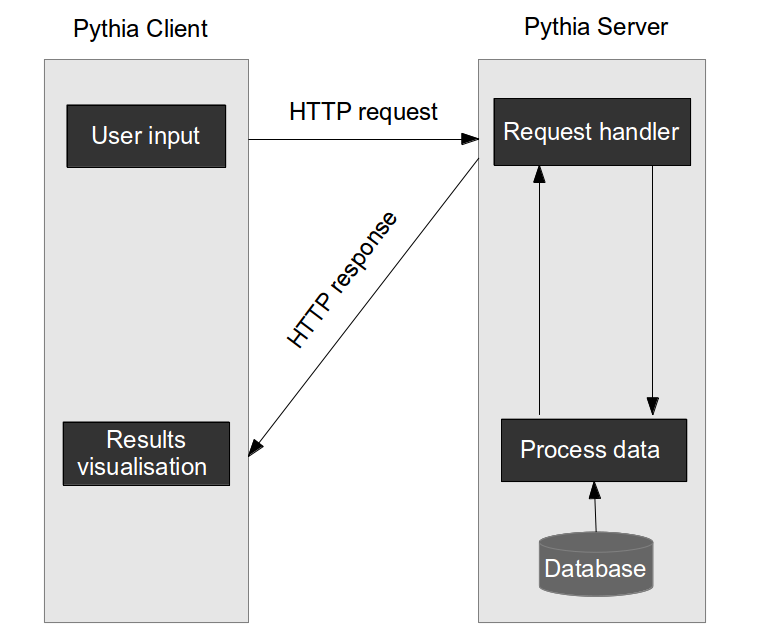
\includegraphics[height=5in, width=6in]{pythia-overview}
    \caption{An overview of Pythia's client-server architecture.}
    \label{PythiaOverview}
  \end{center}
\end{figure} 

\subsection{The Graphical User Interface (GUI) of Pythia}
The motivation behind Pythia is that we wanted to make it as simple as possible for a human to explore and understand events from a Twitter dataset. Therefore, throughout  
the development of Pythia our main consideration was to keep the GUI as lean and simple as possible. The simplicity should not come at the expense of information consumption therefore
another consideration was to give to the user as much information as possible.\\\\
When a user launches Pythia the first page that appears is the one shown in Figure \ref{Pythia1}. A simple text box is used receive the list of keywords provided by the user. The keywords are used to retrieve tweets that contain these words.\\\\
\begin{figure}[htbp]
  \begin{center}
    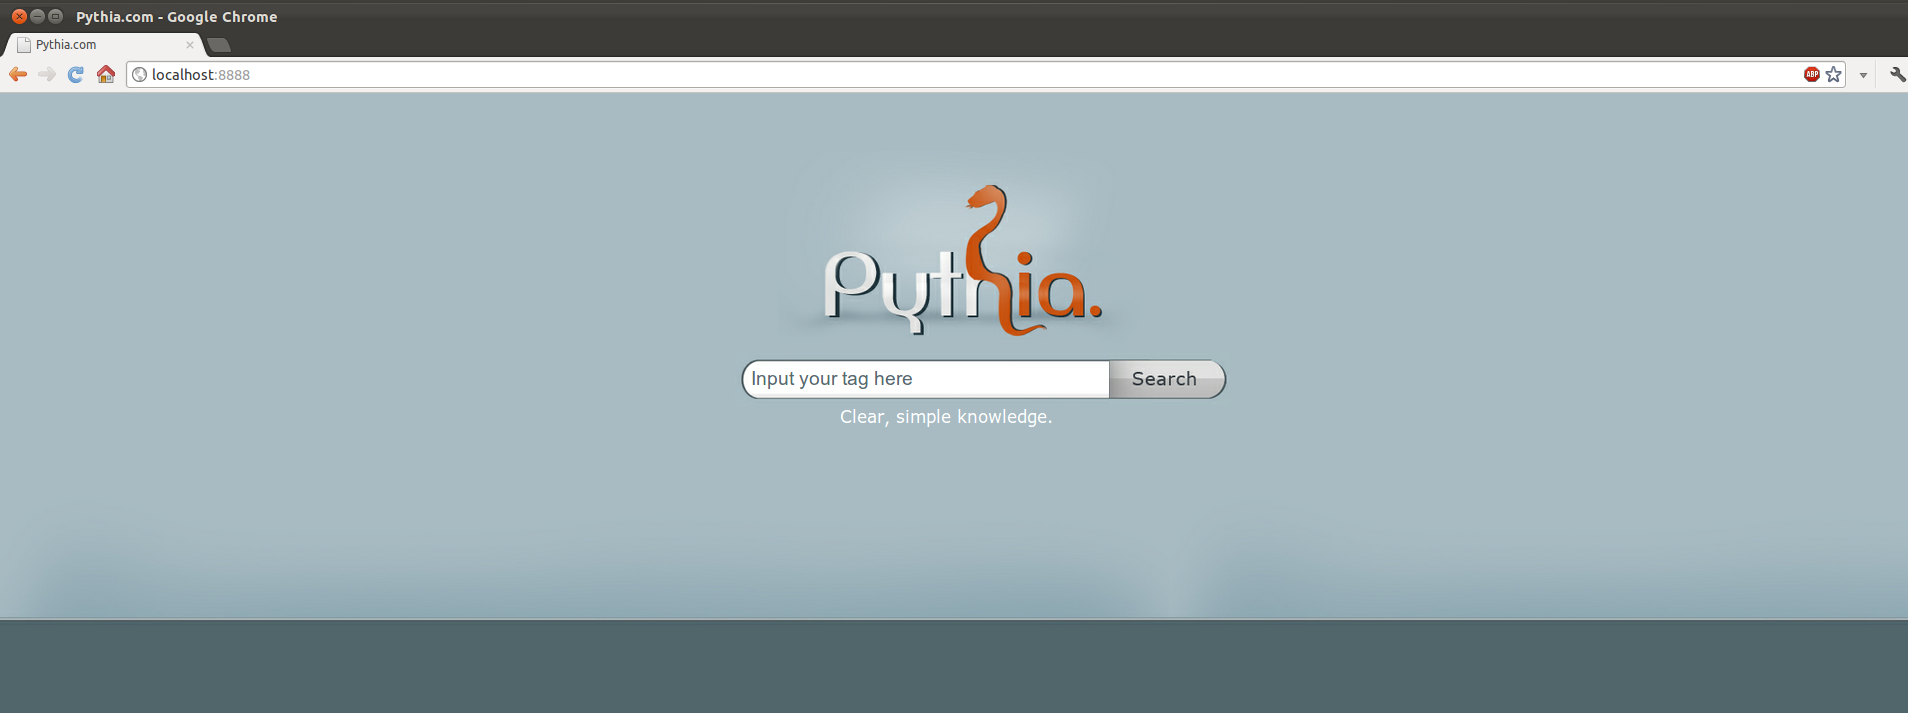
\includegraphics[height=3in, width=6in]{pythia1}
    \caption{The homepage of Pythia. The user inputs in the textbox the keywords related to the events they wish to detect.}
    \label{Pythia1}
  \end{center}
\end{figure} 
The list of keywords is send to the server and the relevan tweets are retrieved from the database. The event detection and summarisation module runs and produces the results which are send back to the user. The detected events appear as small dots on a timeline (Figure \ref{Pythia2}). The x-axis represents time and the y-axis the volume of the tweets in the dataset at that point in time. The smaller timeline on the bottom of the page is a replica of the big one and allows the user to specify a specific time period to zoom in. The timeline allows the user to see the general trend of the events and when they have occured.\\\\    
\begin{figure}[htbp]
  \begin{center}
    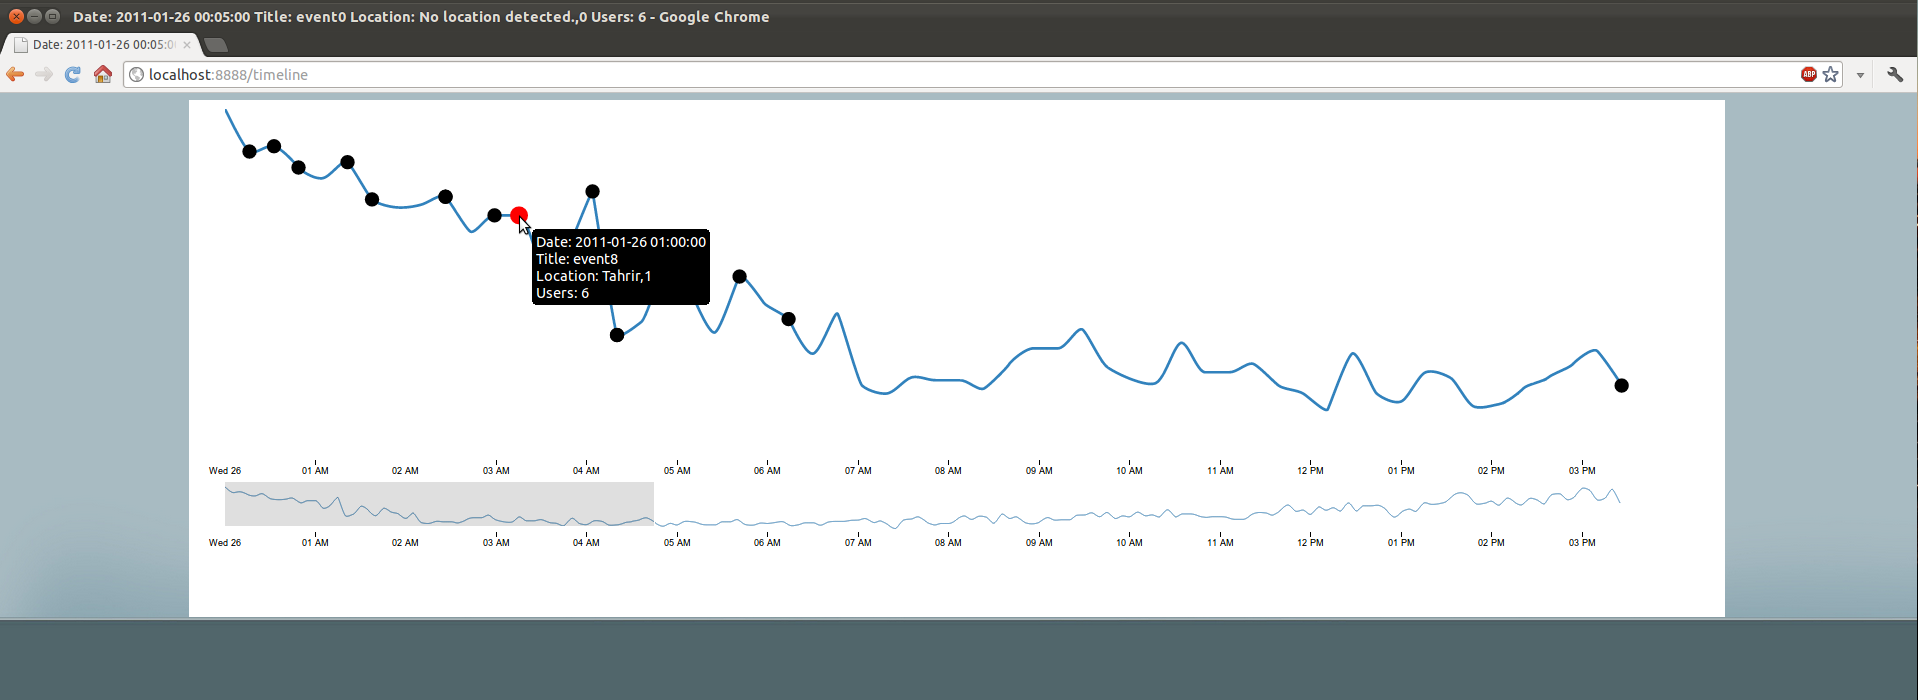
\includegraphics[height=3in, width=6in]{pythia2}
    \caption{The results are presented to the user in the form of an annotated timeline. Each dot on the timeline corresponds to a detected event. The smaller timeline at the bottom of the page allows the    user to zoom in to specific time periods.}
    \label{Pythia2}
  \end{center}
\end{figure} 
In order to understand the events more information is needed. Therefore, we have created a special popup window which displays the results of the summarisation algorithm in a human readable way. This popup window is shown in Figure \ref{Pythia3}. The user can clearly see which tweets have the highest ranking according to the LexRank algorithm and the top keywords related to the event. Additionally, if any named-entities or locations have been identified they are displayed in the relevant sections. Finally, the pie chart in the right hand corner demonstrates the results of the user classification module by showing the proportions of the user types occuring in this event.\\\\    
\begin{figure}[htbp]
  \begin{center}
    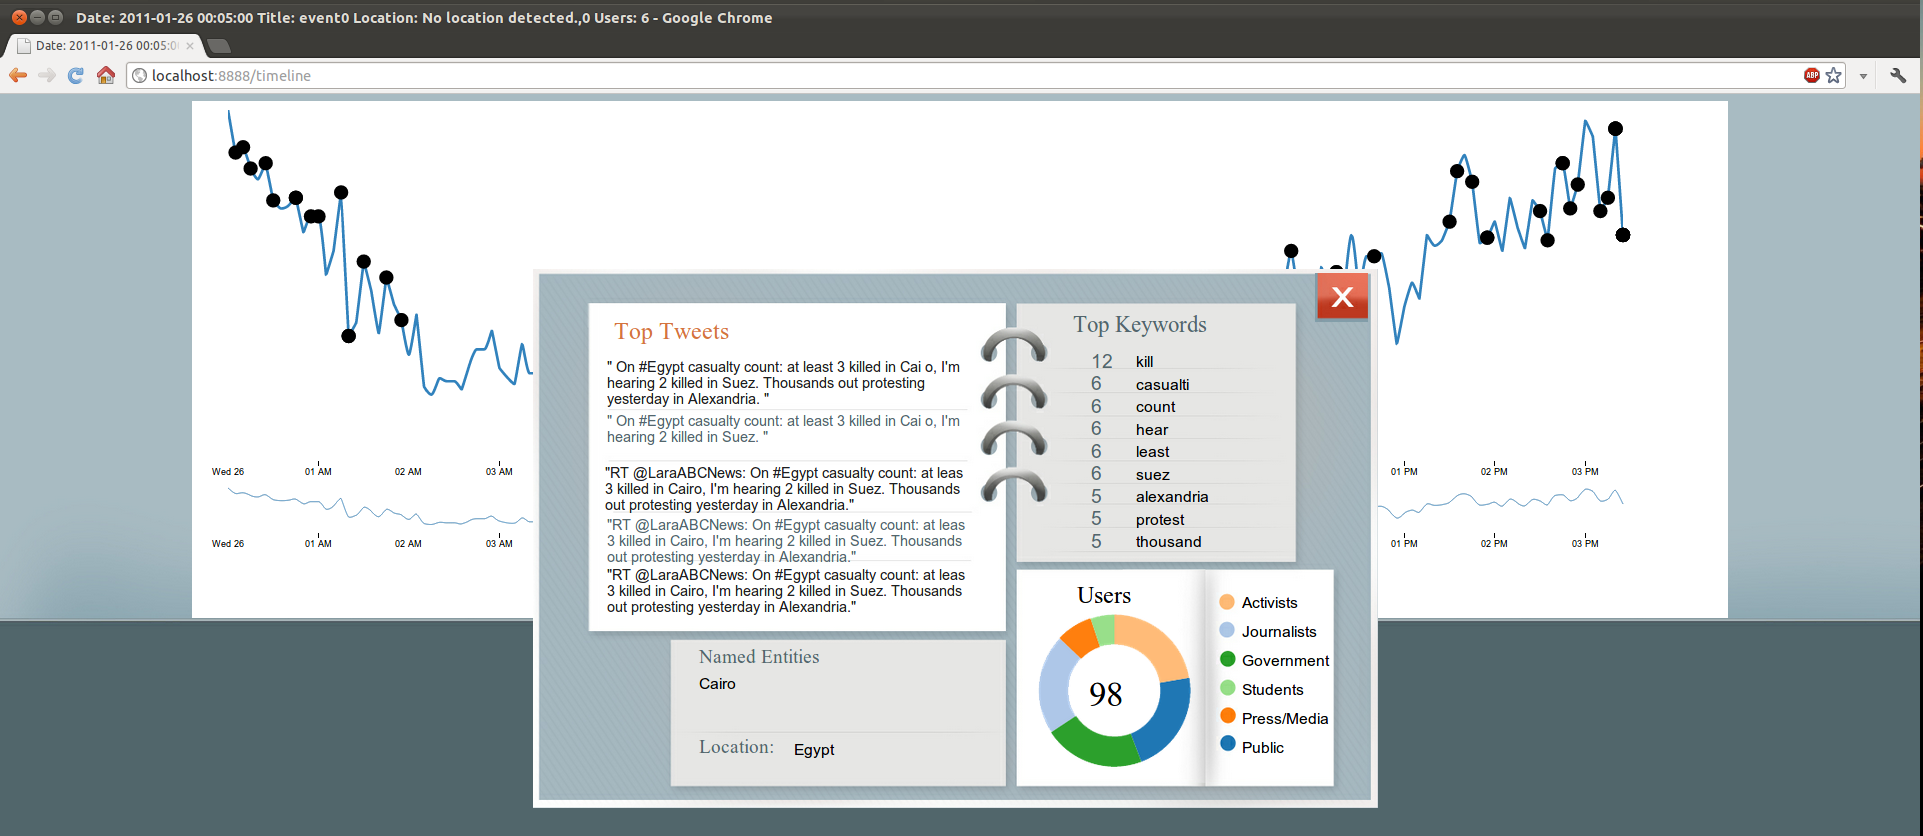
\includegraphics[height=3in, width=6in]{pythia3}
    \caption{The event summary popup helps the user understand what an event is about.}
    \label{Pythia3}
  \end{center}
\end{figure} 

\section{Case studies}
In the next sections we investigate how Pythia performs when it is presented with two different kinds of datasets. Our evaluation is qualitative and it will be based on
the following criteria:
\begin{itemize}
  \item \textbf{Did Pythia detected the expected events?:} In some cases we might be able to have prior knowledge of the existence of some events in the dataset. We need to find out if Pythia is able to retrieve those known events. Even in the case when we do not possess complete prior knowledge about the dataset we expect our system to detect real world-events and not random discussion about the topic. 
  \item \textbf{Is the summary produced by Pythia helpful?:} The purpose of the event summary is to give more information to the user about an event. We evaluate the performance of the summarisation algorithm using the three criteria we set before: relevance, quality, usefulness. 
  \item \textbf{Is Pythia helpful for exploring a historical dataset?:} In general, we must assess if Pythia makes the task of exploring a dataset any easier and if it solves the problem posed by this project.
\end{itemize}\vspace{15pt}

\subsection{Clean dataset}
We first evaluate Pythia using a dataset collected from Twitter for the time period between 25th January 2011 1200pm and 25th January 2011 1220pm. The keywords used to collect the dataset are: 25jan, jan25, egypt, tahrir, mubarak, suez, DownWithMubarak, NOSCAF, SCAF, cairo". The retrieved collection of tweets has been manually processed in order to remove any irrelevant tweets such as spam tweets and discussions. We removed discussions since we want to detect cluster of tweets that describe an event and not meta-discussion about it. The size of the processed dataset is relatively small and it consists of 300 tweets. We have identified 40 different events in the clean dataset and these are the ones we expect Pythia to find. We have given titles to these events and we provide this list of titles in Appendix \ref{Appendix}.\\\\ 
Running Pythia on this clean dataset we get the timeline shown in Figure \ref{Pythia4}. In total, Pythia has detected 36 events out of which 33 are in the list of expected events. The remaining 3 detected events contain combinations of tweets from the other events and therefore we cannot identify which event they describe. Furthermore, the summaries of the events produced mixed results. For all the events that have been correctly detected the top tweets, ranked by the LexRank algorithm, were matching accurately the expected title of the event. However, the named entity recognition algorithm missed some of the named entities in the tweets and it incorrectly identified random words as named entities.    
\begin{figure}[htbp]
  \begin{center}
    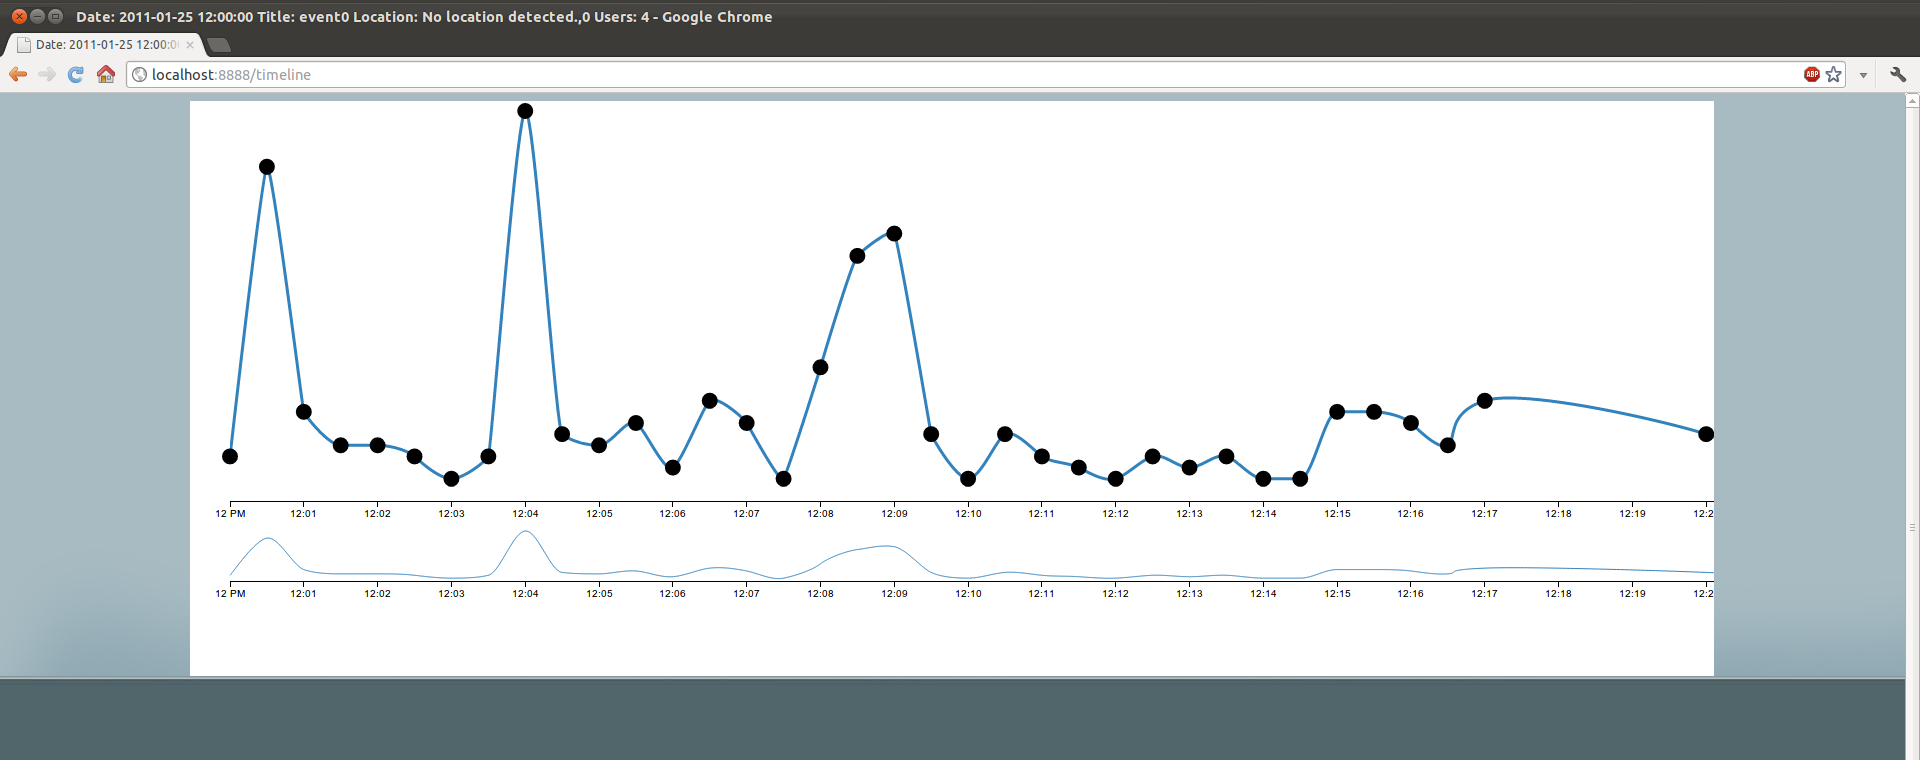
\includegraphics[height=3in, width=6in]{pythia4}
    \caption{The annotated timeline of the detected events for the clean dataset. 31 out of the 40 expected events were detected.}
    \label{Pythia4}
  \end{center}
\end{figure} 

\subsection{Real dataset}
We have seen what Pythia can achieve on a clean dataset but we would like to know its performance on a dataset containing noisy tweets. Noisy tweets are defined as tweets that are either irrelevant to an event or they do not describe an event at all (general discussions between users). In order to compare the results on the noisy dataset with the ones we obtained previously we will use the same dataset as before but now we will not remove the noisy tweets. The timeline for the noisy dataset in Figure \ref{Pythia4} shows that the algorithm detected 45 events. A closer look at the results shows that Pythia has detected 27 of the 40 expected events. The remaining events appear to have different content from the events in our list of expected events. The performance of the summarisation part was the same as for the clean dataset since the ranking algorithms worked very well, unaffected by the noise, in surfacing the most relevant tweets.   
\begin{figure}[htbp]
  \begin{center}
    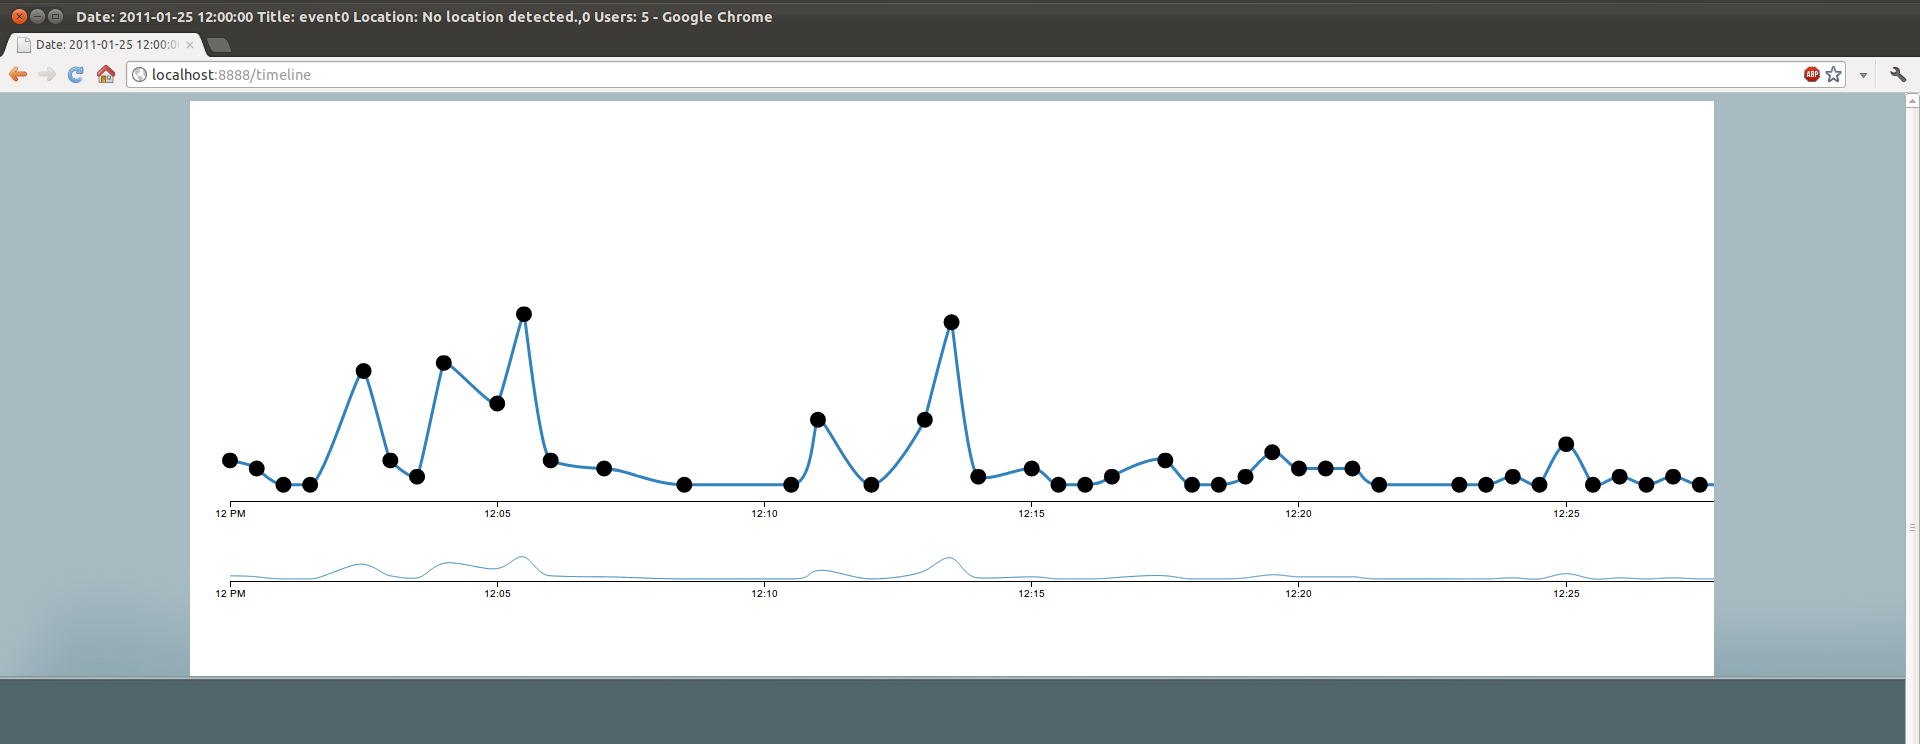
\includegraphics[height=3in, width=6in]{pythia5}
    \caption{The annotated timeline of the detected events for the noisy dataset. 24 out of the 40 expected events were detected.}
    \label{Pythia5}
  \end{center}
\end{figure} 

\subsection{Real dataset with different granularities}
We have carried out some further experiments with Pythia that try to test its performance on a datasets that cover longer time periods. So far we have tried Pythia with datasets that cover smaller time periods. We have run two experiments one with a dataset covering the week starting on 25th January 2011 and another one covering the month starting on 25th January 2011. In the case of the week-long dataset Pythia detected 120 events and for the month-long dataset it detected 320 events. Since these events are far too many to be analysed we decided to select the top ten events according to the ranking given by the metric described in Section \ref{IdentifyEvents}. The most important observation is that as the dataset begins to cover a longer time period Pythia produces more complex and unclear events. More specifically, for the dataset covering a month the top ten events were a mixture of different events and it is extremely hard for a human to identify the specific topic of the event. The reason is because due to the larger size of the dataset the clustering methods accumulate many more tweets in each cluster and the probability of these tweets being irrelevant increases. For the dataset covering a week the problem was as apparent as in the case of the month-long dataset but the events started to become incoherent.      

\section{Summary}


% ------------------------------------------------------------------------


%%% Local Variables: 
%%% mode: latex
%%% TeX-master: "../thesis"
%%% End: 
